\section{Reorder Buffer}\label{capitolo5}
Nei capitoli precedenti abbiamo visto come, sia Tomasulo che lo Scoreboard, prevedano il prelievo delle istruzioni in ordine ma che poi l'esecuzione e il completamento di tali istruzioni avvenga fuori ordine. Ovvero esiste un disaccoppiamento tra il prelevamento e l'esecuzione delle istruzioni. Un altro punto che abbiamo analizzato superficialmente è la risoluzione dei salti, infatti, noi facevamo affidamento sul fatto che il risultato del branch fosse controllato da un'operazione tra interi e che quindi fosse un operazione \emph{veloce}. Nel caso in cui, invece, il ciclo dipenda da un operazione più lenta come una moltiplicazione perdiamo tutti i nostri vantaggi come nel caso del codice seguente:
\begin{verbatim}
Loop:   LD      F0  0   R1
        MULTD   F4  F0  F2
        SD      F4  0   R1
        SUBI    R1  R1  #8
        BNEZ    R1  Loop
\end{verbatim}
Il primo problema è nella predizione del salto, infatti, una corretta previsione diventa fondamentale per mantenere delle buone prestazioni. Oltre alla predizione sui salti l'architettura deve prevedere qualsiasi altro tipo di dipendenza come quella sui dati. Tutte queste predizioni sono effettuate dallo hardware; l'idea di base è quella di prelevare ed eseguire delle istruzioni dipendenti da un salto prima che il risultato di questo salto sia conosciuto, ovvero permettere alle operazioni di essere eseguite fuori ordine ma è necessario che esse siamo completate \emph{in ordine} tutto questo per prevenire che un'operazione venga \emph{committata} prima che tutte le sue precedenti non siano concluse. Questo significa che un'operazione deve essere committata solo quando essa non è più \emph{speculitiva}; il meccanismo che permette questo tipo di controllo è il \emph{ReOrder Buffer (ROB)} che mantiene il risultato delle istruzioni che hanno completato la loro esecuzione ma che non possono essere ancora committate.\\
Il risultato di un salto è predetto e il programma viene eseguito come se la predizione fosse corretta (senza speculazione non si ha la fase di esecuzione). Per fare ciò però sono necessari dei meccanismi per manipolare i casi in cui la predizione è sbagliata. La speculazione hardware permette estende lo scheduling dinamico al di fuori dei blocchi base.\\
La \emph{speculazione hardaware} combina tre idee:
\begin{description}
\item[Dynamic Branch Prediction:] che permette di selezionare quale ramo del salto dovrà essere eseguito prima che il risultato del salto sia conosciuto.
\item[Speculazione:] che permette di eseguire delle istruzioni prima che le dipendenze di controllo siano eseguite.
\item[Scheduling dinamico:] che supporta l'esecuzione fuori ordine ma il completamento in ordine.
\end{description}
Essenzialmente il modello basato sulla speculazione hardware è un modello basato sul \emph{data flow} ovvero, l'esecuzione di un'istruzione inizia quando i suoi operandi sono disponibili.\\
La speculazione hardware è stata introdotta per estendere e supportare l'algoritmo di Tomasulo, in particolare per separare la fase di commit da quella di esecuzione è stato introdotto il \emph{Reorder Buffer}. 
Il meccanismo del \emph{Reorder Buffer} è abbastanza semplice, le istruzioni vengono mantenute in un ordine di tipo FIFO esattamente come vengono prelevate, per ogni record del ROB si mantengono il valore del PC, del registro di destinazione, del risultato e l'eventuale stato dell'eccezione. Quando un'istruzione completa la sua esecuzione il risultato viene inserito nel corrispettivo campo del ROB. Una volta completata l'esecuzione si forniscono i risultati alle altre istruzioni ma si utilizzano i valori dei tag del ROB invece di utilizzare le reservation station. Un'istruzione effettua il commit solo quando è pronta ed è in cima al ROB, solo a quel punto i valori vengono coopiati nei registri.\\
Oltre a questo il Reorder Buffer è comodo per effettuare delle speculazioni, infatti, esso permette di eseguire delle istruzioni senza conseguenze nel caso in cui il branch non sia chiuso; questo meccanismo è chiamato \emph{boosting}. \uppercase{è} l'insieme dell'utilizzo di dynamic scheduling e branch prediction che permette ad un'istruzione di essere eseguita prima che sia conosciuto il valore di un salto.\\
Il fatto di eseguire le istruzioni fuori ordine ma di completarle in ordine permette di prevenire azioni dannose come l'aggiornamento di stati non consistenti o eccezioni.
\subsection{Struttura del reorder buffer}
Come abbiamo detto il reorder buffer mantiene lo stato delle istruzioni che hanno completato la loro esecuzione ma che non sono ancora state committate, inoltre permette di scambiare il risultato di un'istruzione tra le diverse istruzioni in esecuzione. Tutto questo permette un esecuzione delle istruzioni fuori ordine ma un commit di tali istruzioni in ordine. Un esempio di utilizzo del ROB lo abbiamo nell'algoritmo di Tomasulo come mostrato in \figurename\,\ref{fig:tomarob}
\begin{figure}[htb]
\centering
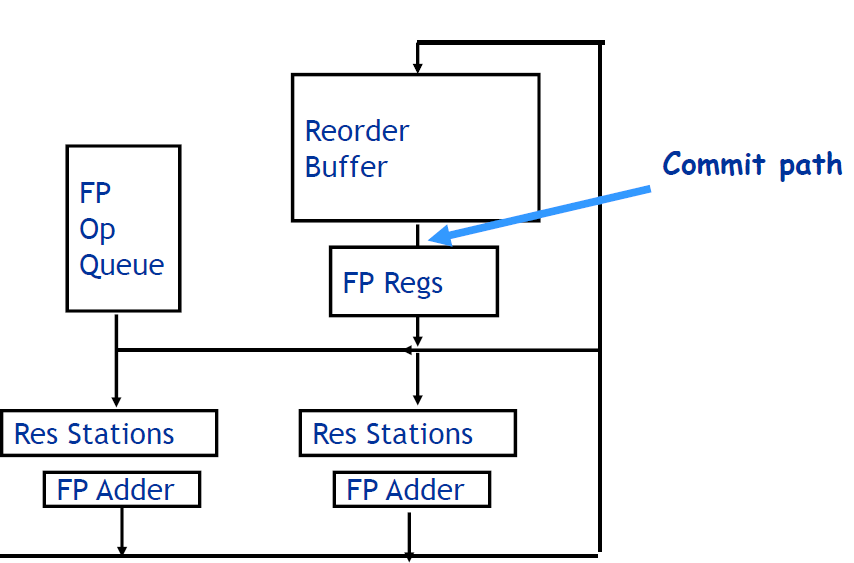
\includegraphics[scale=0.5]{img/tomarob.png}
\caption{Struttura dell'algoritmo di Tomasulo con Reorder Buffer}\label{fig:tomarob}
\end{figure}
Il \emph{Reorder Buffer} rimpiazza completamente lo \emph{Store Buffer}, la funzione di renaming delle \emph{Reservation Station} adesso è effettuata direttamente dal ROB, le RS ora sono utilizzate solamente per immagazzinare istruzioni e operandi da passare alle FU per diminuire gli hazard strutturali.
I puntatori adesso puntano direttamente alle entità del ROB.\\
Ogni entità contenuta nel \emph{Reorder Buffer} contiene a sua volta 4 campi:
\begin{description}
\item[Instruction Type:] Identifica il tipo di istruzione da eseguire.
\item[Destination:] Contiene l'indirizzo del registro di destinazione (ALU e load) o l'indirizzo di memoria (store).
\item[Value:] Mantiene il valore del risultato fino a quando l'istruzione non è committata.
\item[Ready:] Indica che l'istruzione ha completato la sua esecuzione.
\end{description}
LE istruzioni nel Reorder Buffer sono inserite nell'ordine del programma, quando un istruzione viene prelevata essa è allocata in sequenza, essa può essere in tre stati:
\begin{itemize}
\item \textbf{i} issued
\item \textbf{x} in esecuzione
\item \textbf{f} completata
\end{itemize}
Un'istruzione viene committata solo quando tutte le precedenti istruzioni sono state committate e tale istruzione si trova nello stato \textbf{f}.
Il reorder buffer ha una struttura circolare con due puntatori, uno che indica la coda delle istruzioni (punto in cui la successiva istruzione prelevata sarà memorizzata) e uno che ne indica la testa (che tiene traccia della prossima istruzzione da committare). Un esempio di tale struttura è mostrato in \figurename\,\ref{fig:reorderbuff}.
\begin{figure}[htb]
\centering
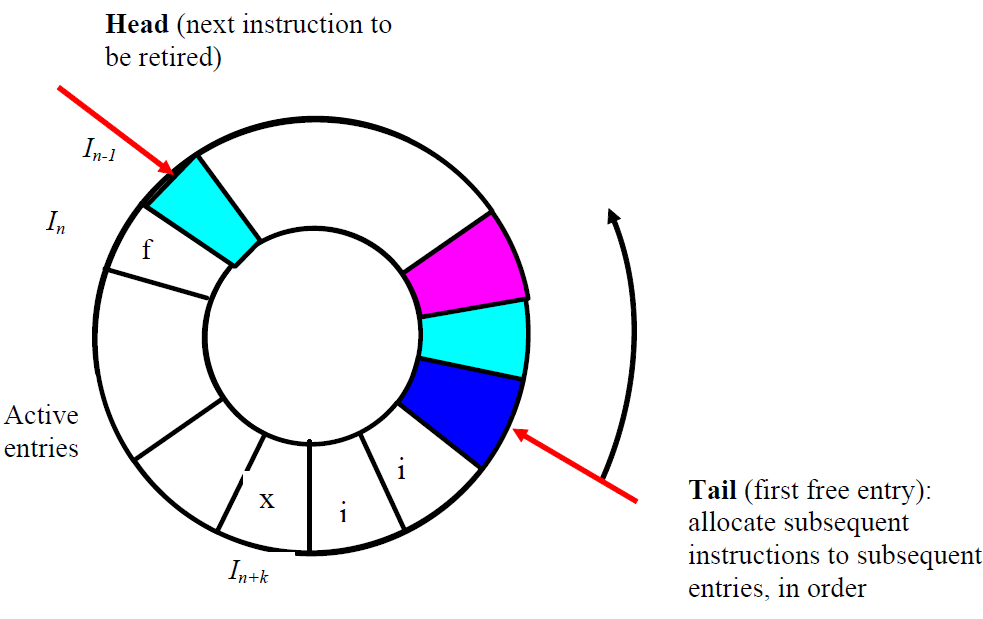
\includegraphics[scale=0.5]{img/reorderbuff.png}
\caption{Struttura di un Reorder Buffer}\label{fig:reorderbuff}
\end{figure}
Nel caso di algoritmo di Tomasulo speculativo con Reorder Buffer i passi dell'algoritmo variano leggermente:
\begin{description}
\item[Issue:] durante questa fase viene prelevata l'istruzione dalla coda delle istruzioni; se il ROB contiene uno slot libeor allora si preleva l'istruzione e si copia nel reorder buffer e nelle reservation station.
\item[Execution:] si eseguono le operazioni sugli operandi, quando sono entrambi disponibili si esegue l'operazione altrimenti si controlla il \emph{Common Data Bus} in attesa dei risultati.
\item[Write Result:] durante questa fase i risultati delle esecuzioni vengono scritti sul CDB e nel ROB inoltre le reservation station vengono marcate come disponibili.
\item[Commit:] vengono aggiornati i diversi registri con il valore contenuto nel ROB, quando l'istruzione puntata dal puntatore di testa del ROB ha completato la sua esecuzione ed è marcata come conclusa allora i dati vengono  copiati nei registri e l'istruzione viene rimossa dal ROB; nel caso di predizione errata le istruzioni vengono cancellate.
\end{description}
Per la fase di commit esistono tre possibili sequenze: 
\begin{enumerate}
\item \textbf{Normal commit:} l'istruzione raggiunge la testa del ROB il risultato è presente nel buffer allora esso viene copiato nei registri e l'istruzione viene rimossa dalla coda.
\item \textbf{Store commit:} come la precedente solo che il risultato viene scritto in memoria anziche nei registri.
\item \textbf{Incorrect prediction:} l'istruzione è un salto la cui predizione è però errata, questo fa si che il ROB sia svuotato e che la predizione ricominci dall'istruzione successiva corretta.
\end{enumerate}
Per quanto riguarda il comportamento delle eccezioni esse sono riconosciute solo quando l'istruzione che genera l'eccezione è committata, questo mantiene il comportamento dell'eccezione.
Per un esempio completo del funzionamento dell'algoritmo di Tomasulo con Reorder Buffer si rimanda alle slide del corso.
\section{Multithreading}\label{capitolo51}
Fino ad ora abbiamo visto il parallelismo intrinseco che esiste tra le istruzioni, ovvero quello che viene comunemente chiamato \emph{ILP}. Il problema dell' ILP è che comporta meccanismi talvolta molto costosi come il \emph{dynamic scheduling} che richiede una grande quantità di logica e limita inoltre il clock.\\
In realtà una macchina ideale dovrebbe avere le seguenti caratteristiche:
\begin{description}
\item[Register renaming:] dovrebbe avere un numero di registri infinito più un meccanismo di buffering degli operandi per evitare tutti i problemi di WAW e WAR.
\item[Branch prediction (\emph{perfetta}):] ovvero una predizione dei salti che non commette errori e una lista illimitata di istruzioni da poter eseguire.
\item[Memory-address alias analysis:] gli indirizzi sono conosciuti e le \emph{store} possono effettuare le loro operazioni prima che le load provino che gli indirizzi non sono uguali.
\item[Unlimited issue:] la CPU può prelevare un numero di istruzioni arbitrario per ogni ciclo di clock, ricercando tali istruzioni in qualsiasi punto del codice.
\item[One cycle latency for all instruction:] tutte le istruzioni hanno un solo ciclo di latenza questo comporta che ogni istruzione dipendente può essere schedulata nel ciclo successivo.
\item[Perfect cache:] tutte le \emph{load} e le \emph{store} vengono eseguite in un singolo ciclo di clock e non avvengono mai \emph{cache miss.}
\end{description}
Oltre a queste caratteristiche fisiche una macchina ideale deve anche disporre di uno \emph{scheduling dinamico perfetto} il che comporta il fatto di poter prelevare le istruzioni in modo arbitrariamente lontano, la possibilità di rinominare tutti i registri, la capacità di determinare quali dipendenze dati esistono nel set di istruzioni prelevato ed infine fornire un numero adeguato di unità funzionali replicate per poter eseguire tutte le istruzioni pronte.\\
In realtà nelle CPU attualmente in commercio non si possono avere più di due riferimenti a memoria per ciclo, inoltre vi sono alcune limitazioni sul numero di bus e sul numero di porte del \emph{register file}; tutte queste limitazioni definiscono un limite al numero di operazioni che può essere prelevato durante un singolo ciclo di clock.\\
Appena introdotto i processori superscalari erano di tipo 2-issue e si  velocemente in processori  4-issue. Attualmente possiamo trovare molto raramente dei processori 6-issue ma non superiori in quanto risulta molto complicato decidere 8 o più istruzioni indipendenti da eseguire ad ogni ciclo, il calcolo è molto complesso e la frequenza del processore dovrebbe essere diminuita. Gli svantaggi dei processori superscalari sono la grande quantità di logica necessaria per decidere l'indipendenza delle istruzioni, ed inoltre, non è scalare infatti per aumentare la finestra di prelevamento è necessario ridurre la frequenza di clock.
\subsection{Processori embedded}
Al contrario dei processori superscalari i processori pensati per prodotti embedded devono essere economici e consumare poco energia. La maggior parte dei processori per i sistemi embedded è progettata da:
\begin{itemize}
\item ARM
\item STMicroelectronics
\end{itemize}
\paragraph{ARM Cortex-A8}
Basato sull'architettura ARMv7 è il processore presente sul System-on-Chip A4 di Apple. \uppercase{è} un processore di tipo dual-issue con esecuzione in ordine. Utilizzato nel SoC A4 con manifattura a 45nm e frequenza di 1GHz è stato utilizzato nel primo iPad, sull'iPhone4 e sull'iPod Touch.
\paragraph{ARM Cortex-A9}
Basato sull'architettura ARMv7 è un processore di tipo dual core presente sul System-on-Chip A5 di Apple. \uppercase{è} un processore di tipo dual-issue con esecuzione in ordine. Utilizzato nel SoC A5 con manifattura a 45nm e successivamente 35nm e frequenza di 1GHz è stato utilizzato nell'iPad2, sull'iPhone 4S e sull'iPad Mini e sulle Apple TV di terza generazione.
\paragraph{Apple A6 SoC}
Il SoC A6 è stato introdotto nel settembre 2012 per l'arrivo dell' iPhone5 è basato sull'architettura ARMv7 personalizzata da Apple, comprende un processore dual core da 1.3GHz e un GPU triple-core PowerVR SGX, inoltre incorpora una RAM da 1GB LPDDR2-1066 che permette di incrementare la banda di memoria teorica fino ad un valore di 8.5 GB/s
Confrontando due processori Intel possiamo vedere come per quanto riguarda i sistemi embedded lo scopo principale sia quello di mantenere contenuto il consumo di energia, infatti:
\begin{itemize}
\item Intel i7 920: processore a 4 cores a 2.66 GHz; consumo medio di energia \textbf{130W}
\item Intel Atom 230 (\emph{embedded}): 1 core a 1.66 GHz; consumo medio di energia \textbf{4W}
\end{itemize}
Il problema per i sistemi embedded è trovare il giusto compromesso tra risparmio di energia e performance. Per fare questo utilizzano, a differenza dei sistemi \emph{general purpose}, uno \emph{scheduling statico} ovvero uno scheduling effettuato a \emph{compile-time} e le istruzioni di tipo VLIW. Questo meccanismo permette di decidere quando e dove eseguire le istruzioni durante la compilazione del programma. Questo permette di ridurre il design dell'hardware.\\
Le difficoltà che si riscontrano sono tuttavia molteplici e diverse, ad esempio, il compilatore deve essere molto evoluto per individuare il parallelismo tra le istruzioni e schedularle sulle diverse unità funzionali. Inoltre, esiste una \emph{incompatibilità binaria} a causa delle ottimizzazioni architetturali che effettua il compilatore.
\subsection{Multithreading e Multiprocessing}
Un'alternativa per incrementare le performance è quella di sfruttare il parallelismo dei \emph{thread} al posto del semplice ILP.
Un \emph{thread} è parte di un processo con istruzioni e dati propri, esso può essere parte di un programma con molti processi oppure può essere un programma indipendente; ogni thread ha un suo \emph{stato} necessario per la sua esecuzione. Un esempio di come un thread può esistere è mostrato in \figurename\,\ref{fig:threadproc}.
\begin{figure}[htb]
\centering
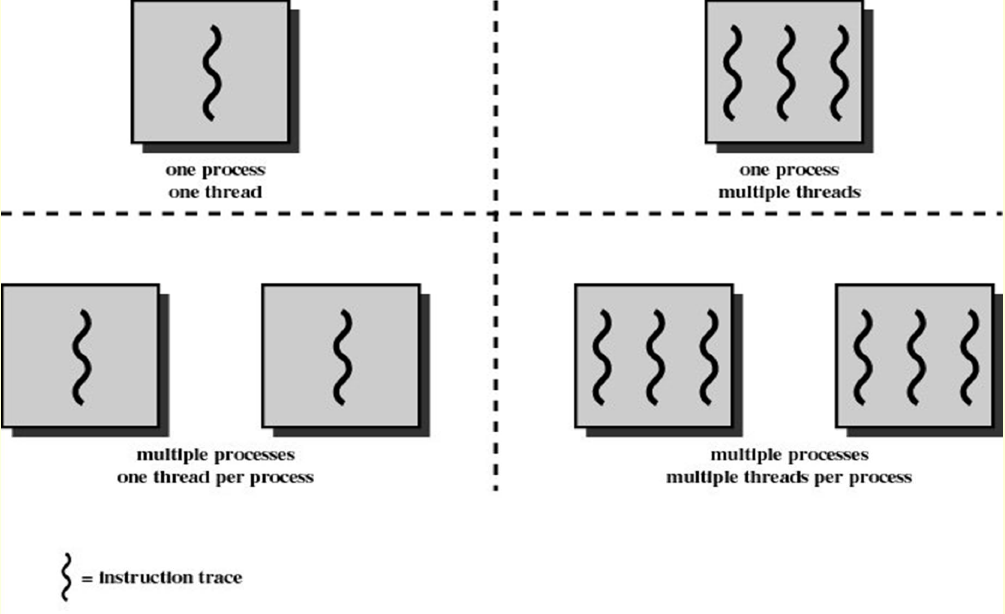
\includegraphics[scale=0.5]{img/threadproc.png}
\caption{Esempio di esistenza dei thread}\label{fig:threadproc}
\end{figure}
I thread vengono creati dai programmatori o dal sistema operativo, ad ogni thread viene associata una specifica porzione di computazione che può essere formata da poche istruzioni oppure da molte righe di codice. Un processo scambia tra i diversi thread, quando uno va in stallo un altro va in esecuzione, lo stato di ogni thread deve essere salvato mentre un altro thread è in esecuzione; sono così necessari register file e PC multipli.\\
Il multithreading permette a più thread di condividere le unità funzionali di un singolo processore, lo spazio degli indirizzi di memoria è condiviso attraverso meccanismi di memoria virtuale, l'HW supporta l'abilità di cambiare tra i diversi threads in modo veloce e più efficentemente di quanto si possa fare in uno scambio di contesto tra processi.\\
Esistono diversi tipi di multithreading in ambienti superscalari.
\begin{description}
\item[Coarse-grained:] meccanismo che prevede che quando un thread si blocca, ad esempio per una lettura del disco, un altro thread va in esecuzione.
\item[Fine-grained:] il switching tra i diversi thread è effettuato ad ogni istruzione
\item[Simultaneous:] più thread utilizzano slot di prelevamento multipli in un singolo ciclo di clock.
\end{description}
Analizziamo ora i diversi tipi di multithreading partendo dal caso di un processore superscalare senza multithreading; l'utilizzo degli \emph{issue slot} è limitato dalla mancanza di ILP, inoltre nel nostro esempio abbiamo anche uno stallo dovuto ad una cache miss che lascia il programma in sospeso. Il nostro esempio è mostrato in \figurename\,\ref{fig:normalth}
\begin{figure}[htb]
\centering
\subfigure[normalth]{
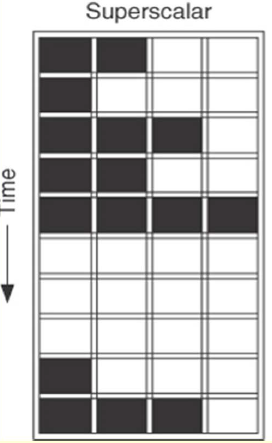
\includegraphics[scale=0.4]{img/normalth.png}
\label{fig:normalth}
}
\subfigure[coarse grained]{
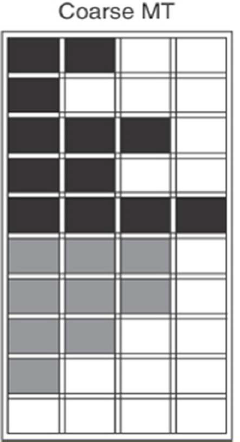
\includegraphics[scale=0.4]{img/croasgrained.png}
\label{fig:croasgrained}
}
\caption{Esempio di processore superscalare \ref{fig:superscalar} e di processore superscalare con multithreading di tip coarse-grained \ref{fig:croasgrained}}
\end{figure}
Nel caso di multithreading superscalare di tipo coarse-grained come quello in \figurename	\,\ref{fig:croasgrained} i lunghi stalli vengono nascosti mandando in esecuzione un nuovo thread che occupi le risorse del processore, questo meccanismo riduce il numero di cicli in cui il processore è inattivo; tuttavia le limitazioni dovute alle ILP continuano a far si che alcuni slot siano vuoti, quando c'è uno stallo è necessario svuotare la pipeline prima di iniziare con il nuovo thread, inoltre il nuovo thread necessita di un periodo di start-up nel quale non si completano operazioni e si riduce perciò il throughtput del sistema. Date queste limitazioni il coarse-grained MT è applicabile solo quando il tempo per il riempimento della pipeline è molto minore dei tempi di stallo.\\
Un'alternativa al coarse-grained è il \emph{fine-grained multithreading} in questo caso il MT preleva un istruzione da un thread diverso ad ogni ciclo, ovvero l'esecuzione di thread multipli viene intervallata in un circolo \emph{round-robin} e si saltano quei thread che sono bloccati. Il processore deve essere in grado di cambiare thread ad ogni ciclo ma questo permette di nascondere gli stalli mandando in esecuzione altri thread e non considerando quello bloccato. Tuttavia il tempo di esecuzione di un thread è rallentato perchè un thread pronto deve comunque aspettare l'esecuzione di altri thread. Anche in questo caso inoltre abbiamo degli issue slot vuoti dovuti alla limitazione dell'ILP. Un esempio di \emph{fine-grained MT} è mostrato in \figurename\,\ref{fig:finegrained}
\begin{figure}[htb]
\centering
\subfigure[finegrained]{
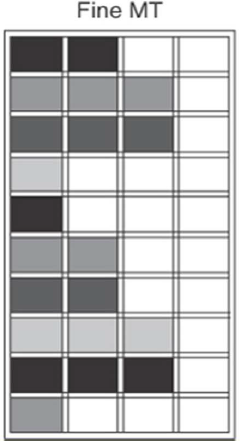
\includegraphics[scale=0.4]{img/finegrained.png}
\label{fig:finegrained}
}
\subfigure[simultaneousmt]{
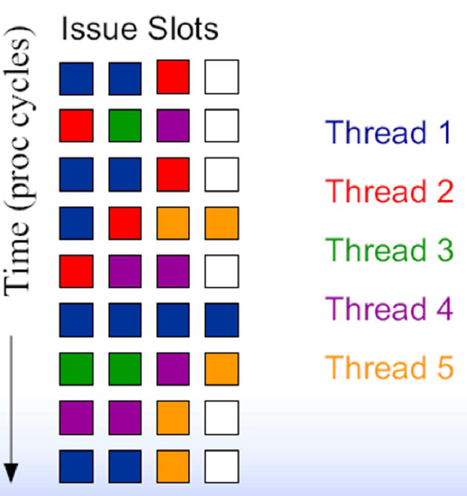
\includegraphics[scale=0.4]{img/simultaneousmt.png}
\label{fig:simultaneousmt}
}
\caption{Esempio di fine-grained MT \ref{fig:finegrained} e di simultaneous MT \ref{fig:simultaneousmt}}
\end{figure}
Un esempio del \emph{fine-grained multithread} è il \textbf{Sun Niagara T1} un processore ad 8 core nel quale un singolo core può gestire fino ad un massimo di 4 thread  per un totale di 32 thread gestiti. Ad ogni ciclo di clock ogni core esegue un thread diverso tra i quattro disponibili. Quando un thread è bloccato il core sul quale è eseguito manda in esecuzione un altro thread solo quando tutti e quattro i thread di un core sono bloccati allora il core risulta in stallo.\\
In pratica il multithreading permette di nascondere eventi di latenze molto lunghe e mantenere occupate le unità funzionali.\\
A questo punto però ci chiediamo perchè non sfruttare sia ILP che il TLP contemporaneamente. Per fare questo utiliziamo il \emph{simultaneous multithreading} come mostrato in \figurename\,\ref{fig:simultaneousmt}. In questo meccanismo più thread utilizzano i diversi issue slot nello stesso ciclo di clock, la risoluzione delle dipendenze avviene tramite scheduling dinamico, il register renaming permette di utilizzare identificativi univoci per mischiare istruzioni provenienti da thread diversi. L'utilizzo degli issue slot è limitato solo dalla loro occupazione. L'unico difetto di questa tecnica è che inevitabilmente si compromette il tempo di esecuzione del singolo thread.
Il fattore principale che ha spinto l'introduzione del SMT è il fatto che le CPU moderne hanno più unità funzionali di quanto un singolo thread può sfruttare, tale implementazione è la più comune nei processori Intel Core i7.\\
Per implementare tale meccanismo bisogna però migliorare anche l'unità di \emph{Fetch} in quanto essa deve essere in grado di prelevare le istruzioni da più thread ed inoltre decidere da quali thread prelevare. I vantaggi di questa tecnica sono i ridotti salti non risolti, i minori problemi di load miss ed infine la minore quantità di istruzioni in coda.